\chapter{The Compact Muon Solenoid Detector}
\label{chap:CMS}

The \ac{CMS} detector~\cite{CMS:2008xjf} is one of the two general-purpose detectors involved in the discovery of the Higgs boson in 2012~\cite{ATLAS:2012yve,CMS:2012qbp}. It is located around 100 meters underground near the French town of Cessy. The full detector weights over 14 thousand tones, and is roughly cylindrically symmetric with a length and diameter of 21 and 15 meters, respectively. It consists of several layers of subsystems, as illustrated in Figure~\ref{fig:CMS}.

\begin{figure}[tbh!]
 \begin{center}
 \begin{tabular}{c}
 \includegraphics[width=0.9\textwidth]{figures/Part2/CMS/cms}
 \end{tabular}
 \caption{A sectional view of the \ac{CMS} detector, adapted from~\cite{Sakuma:2013jqa}.}
 \label{fig:CMS}
 \end{center}
\end{figure}

Brief descriptions of these subsystems are given in \autoref{sec:TK}-\autoref{sec:TrigSys}. The coordinate system adopted by \ac{CMS} is introduced in \autoref{sec:Coord}.

\section{Coordinate System Used in the CMS Detector}
\label{sec:Coord}

As illustrated in Figure~\ref{fig:axis3D}, the coordinate system adopted by \ac{CMS} uses the nominal \ac{IP} as its origin, with the $x$-axis pointing radially inward towards the center of the \ac{LHC} ring, the $y$-axis pointing vertically upward towards the sky, and the z-axis pointing along the beam line towards west of the detector.

\begin{figure}[tbh!]
 \begin{center}
 \begin{tabular}{c}
 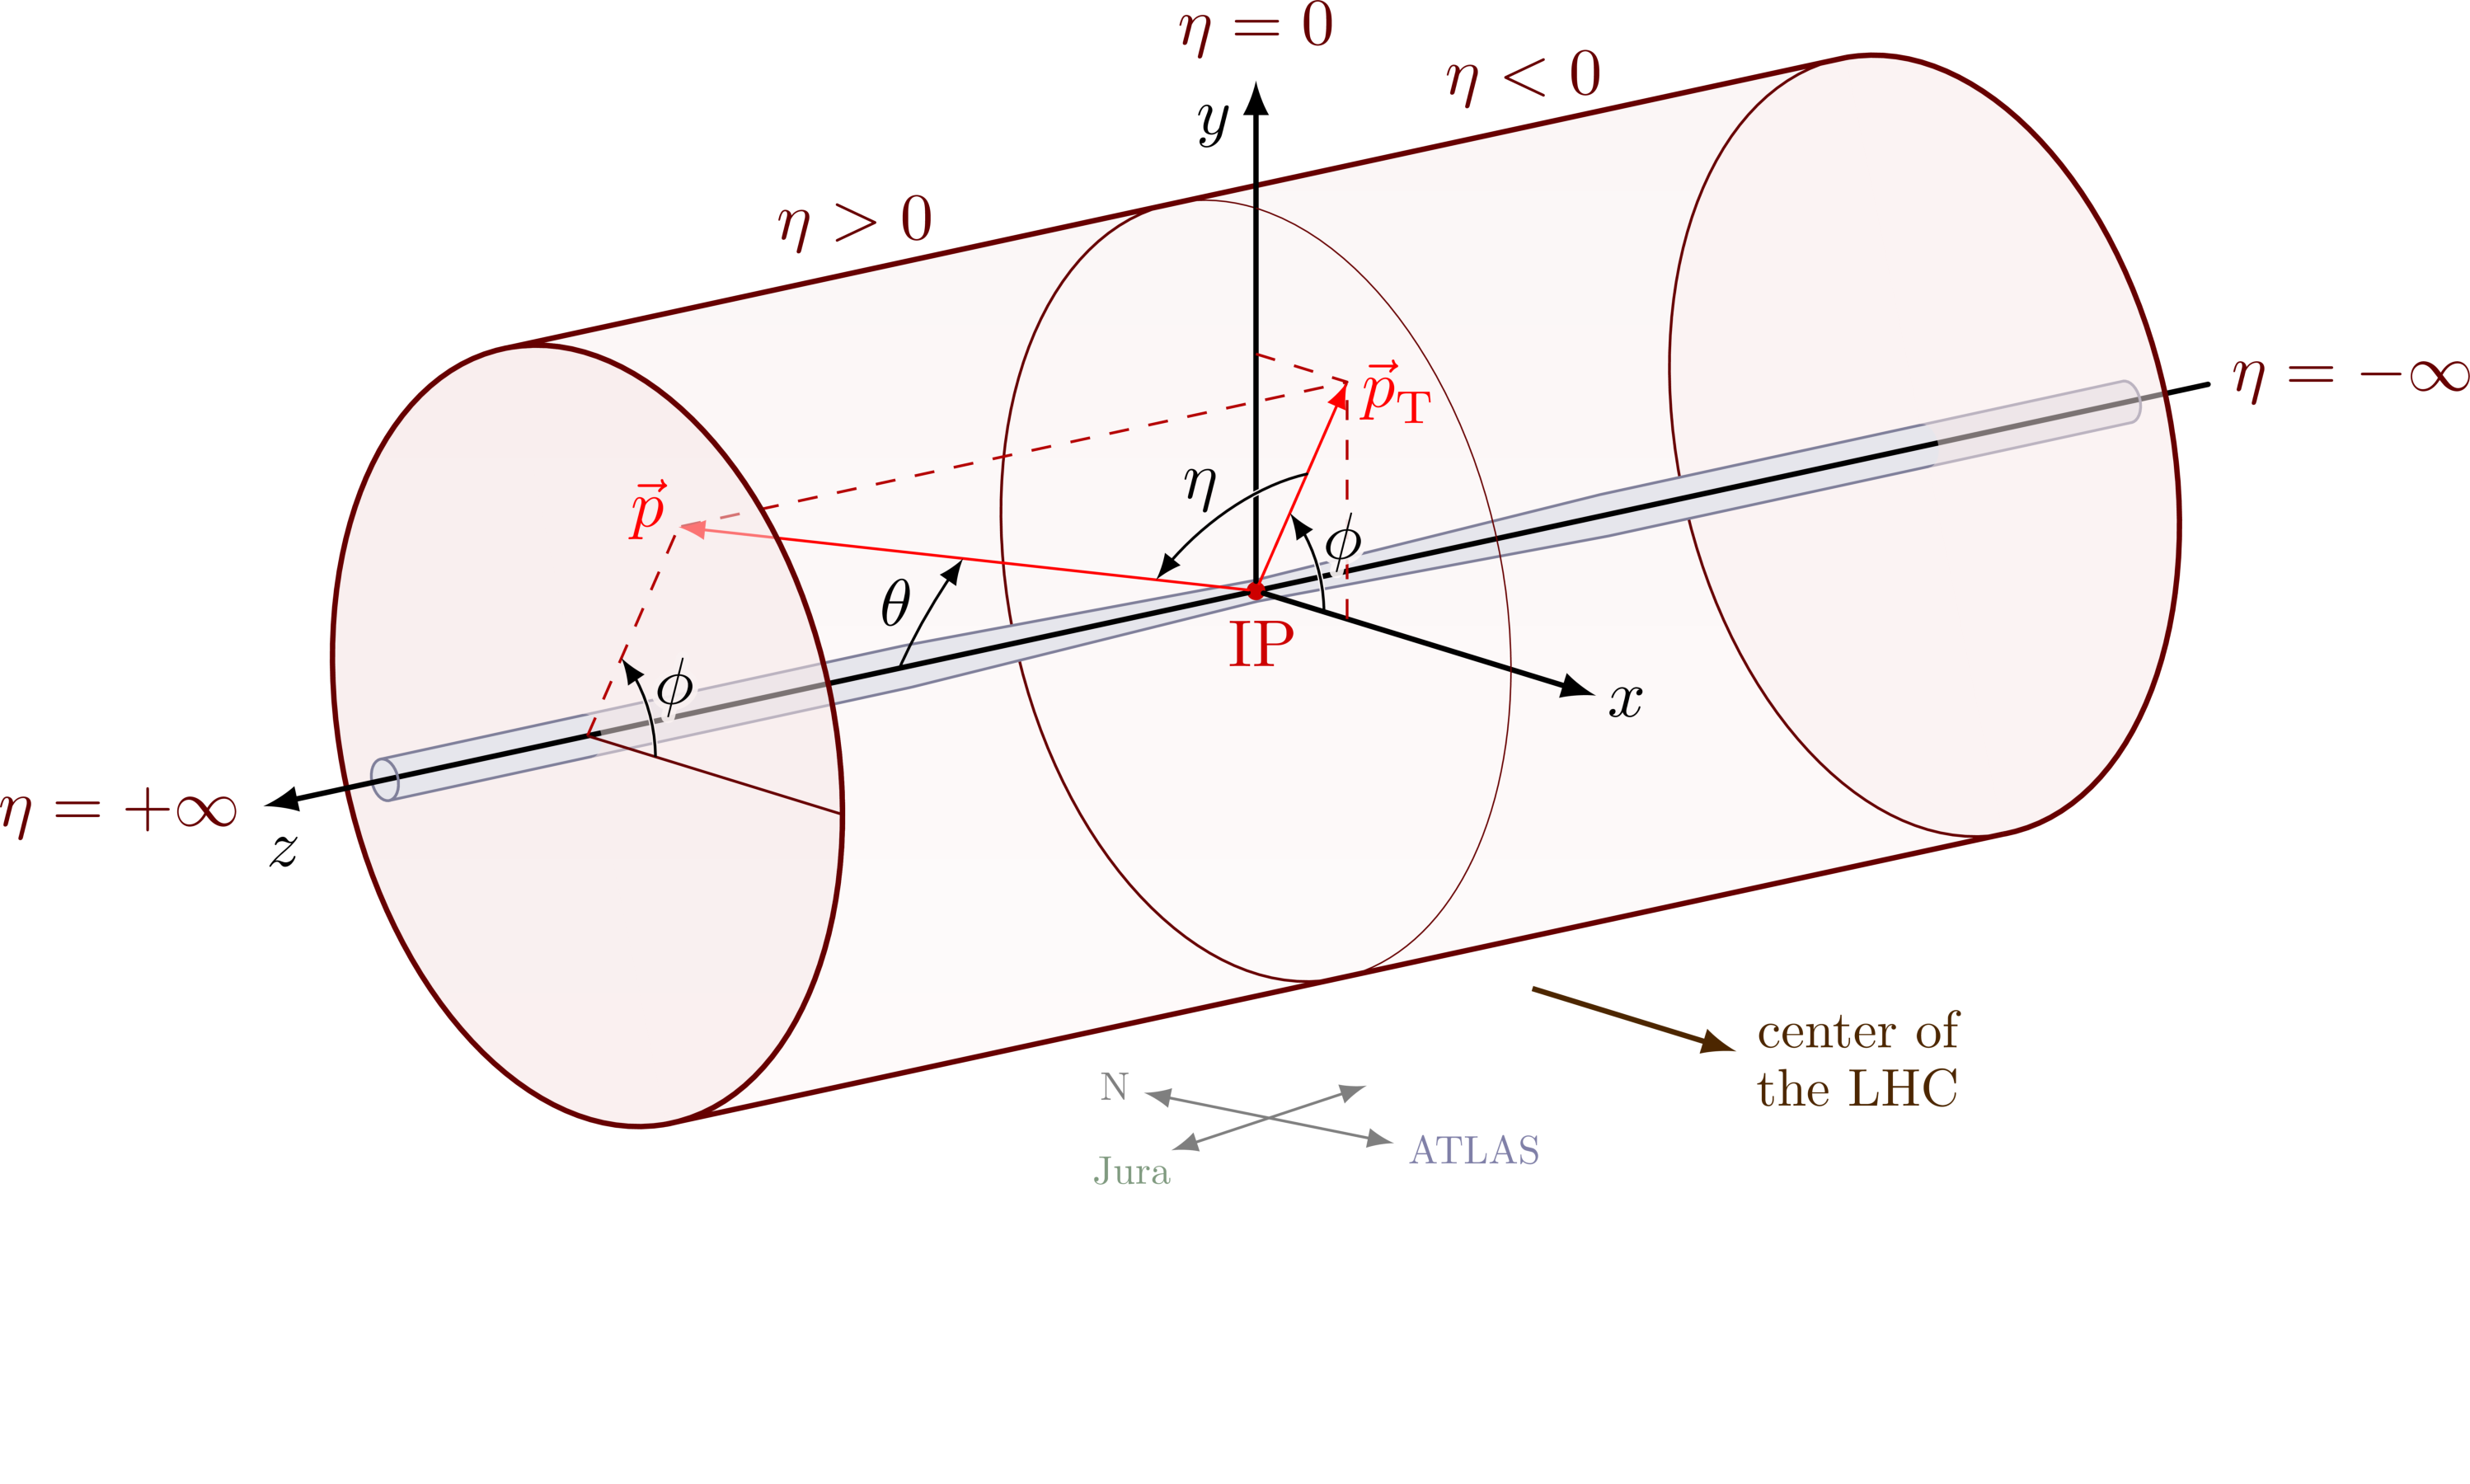
\includegraphics[width=0.8\textwidth]{figures/Part2/CMS/axis3D_CMS-004}
 \end{tabular}
 \caption{A sketch of the coordinate system adopted by \ac{CMS}, adapted from~\cite{tikz:3D}.}
 \label{fig:axis3D}
 \end{center}
\end{figure}

The $x$- and $y$-axis form the transverse plane as they are both orthogonal to the beam line (z-axis). The distance from the \ac{IP} in the transverse plane is defined as $r=\sqrt{x^2+y^2}$. Variables defined entirely in the transverse plane, such as $\pt$, \MET, and $\Ht$, are often indicated by a subscripted T. The azimuthal angle $\phi$ is measured from the positive $x$-axis and the polar angle $\theta$ is measured from the positive z-axis. Another variable $\eta$, known as pseudorapidity, is defined as

\begin{equation}
\eta=-\ln(\frac{\theta}{2}) 
\end{equation}
or alternatively 
\begin{equation}
\eta=\frac{1}{2}\ln(\frac{p+p_z}{p-p_z}).
\label{eq:eta}
\end{equation}

It is preferred over $\theta$ mainly due to: i) particle production rate is roughly uniform in this variable, and ii) a difference in this variables, denoted by $\mathrm{\Delta}\eta$, is invariant under Lorentz boosts. The conversion between $\eta$ and $\theta$ is illustrated in Figure~\ref{fig:axis2D}. The $\mathrm{\Delta}\eta$ and the difference in azimuthal angles, denoted by $\mathrm{\Delta}\phi$, are used to define the distance parameter $\mathrm{\Delta}R$

\begin{equation}
\label{eq:DR}
\mathrm{\Delta}R=\sqrt{\mathrm{\Delta}\eta^2+\mathrm{\Delta}\phi^2}.
\end{equation}

\begin{figure}[tbh!]
 \begin{center}
 \begin{tabular}{c}
 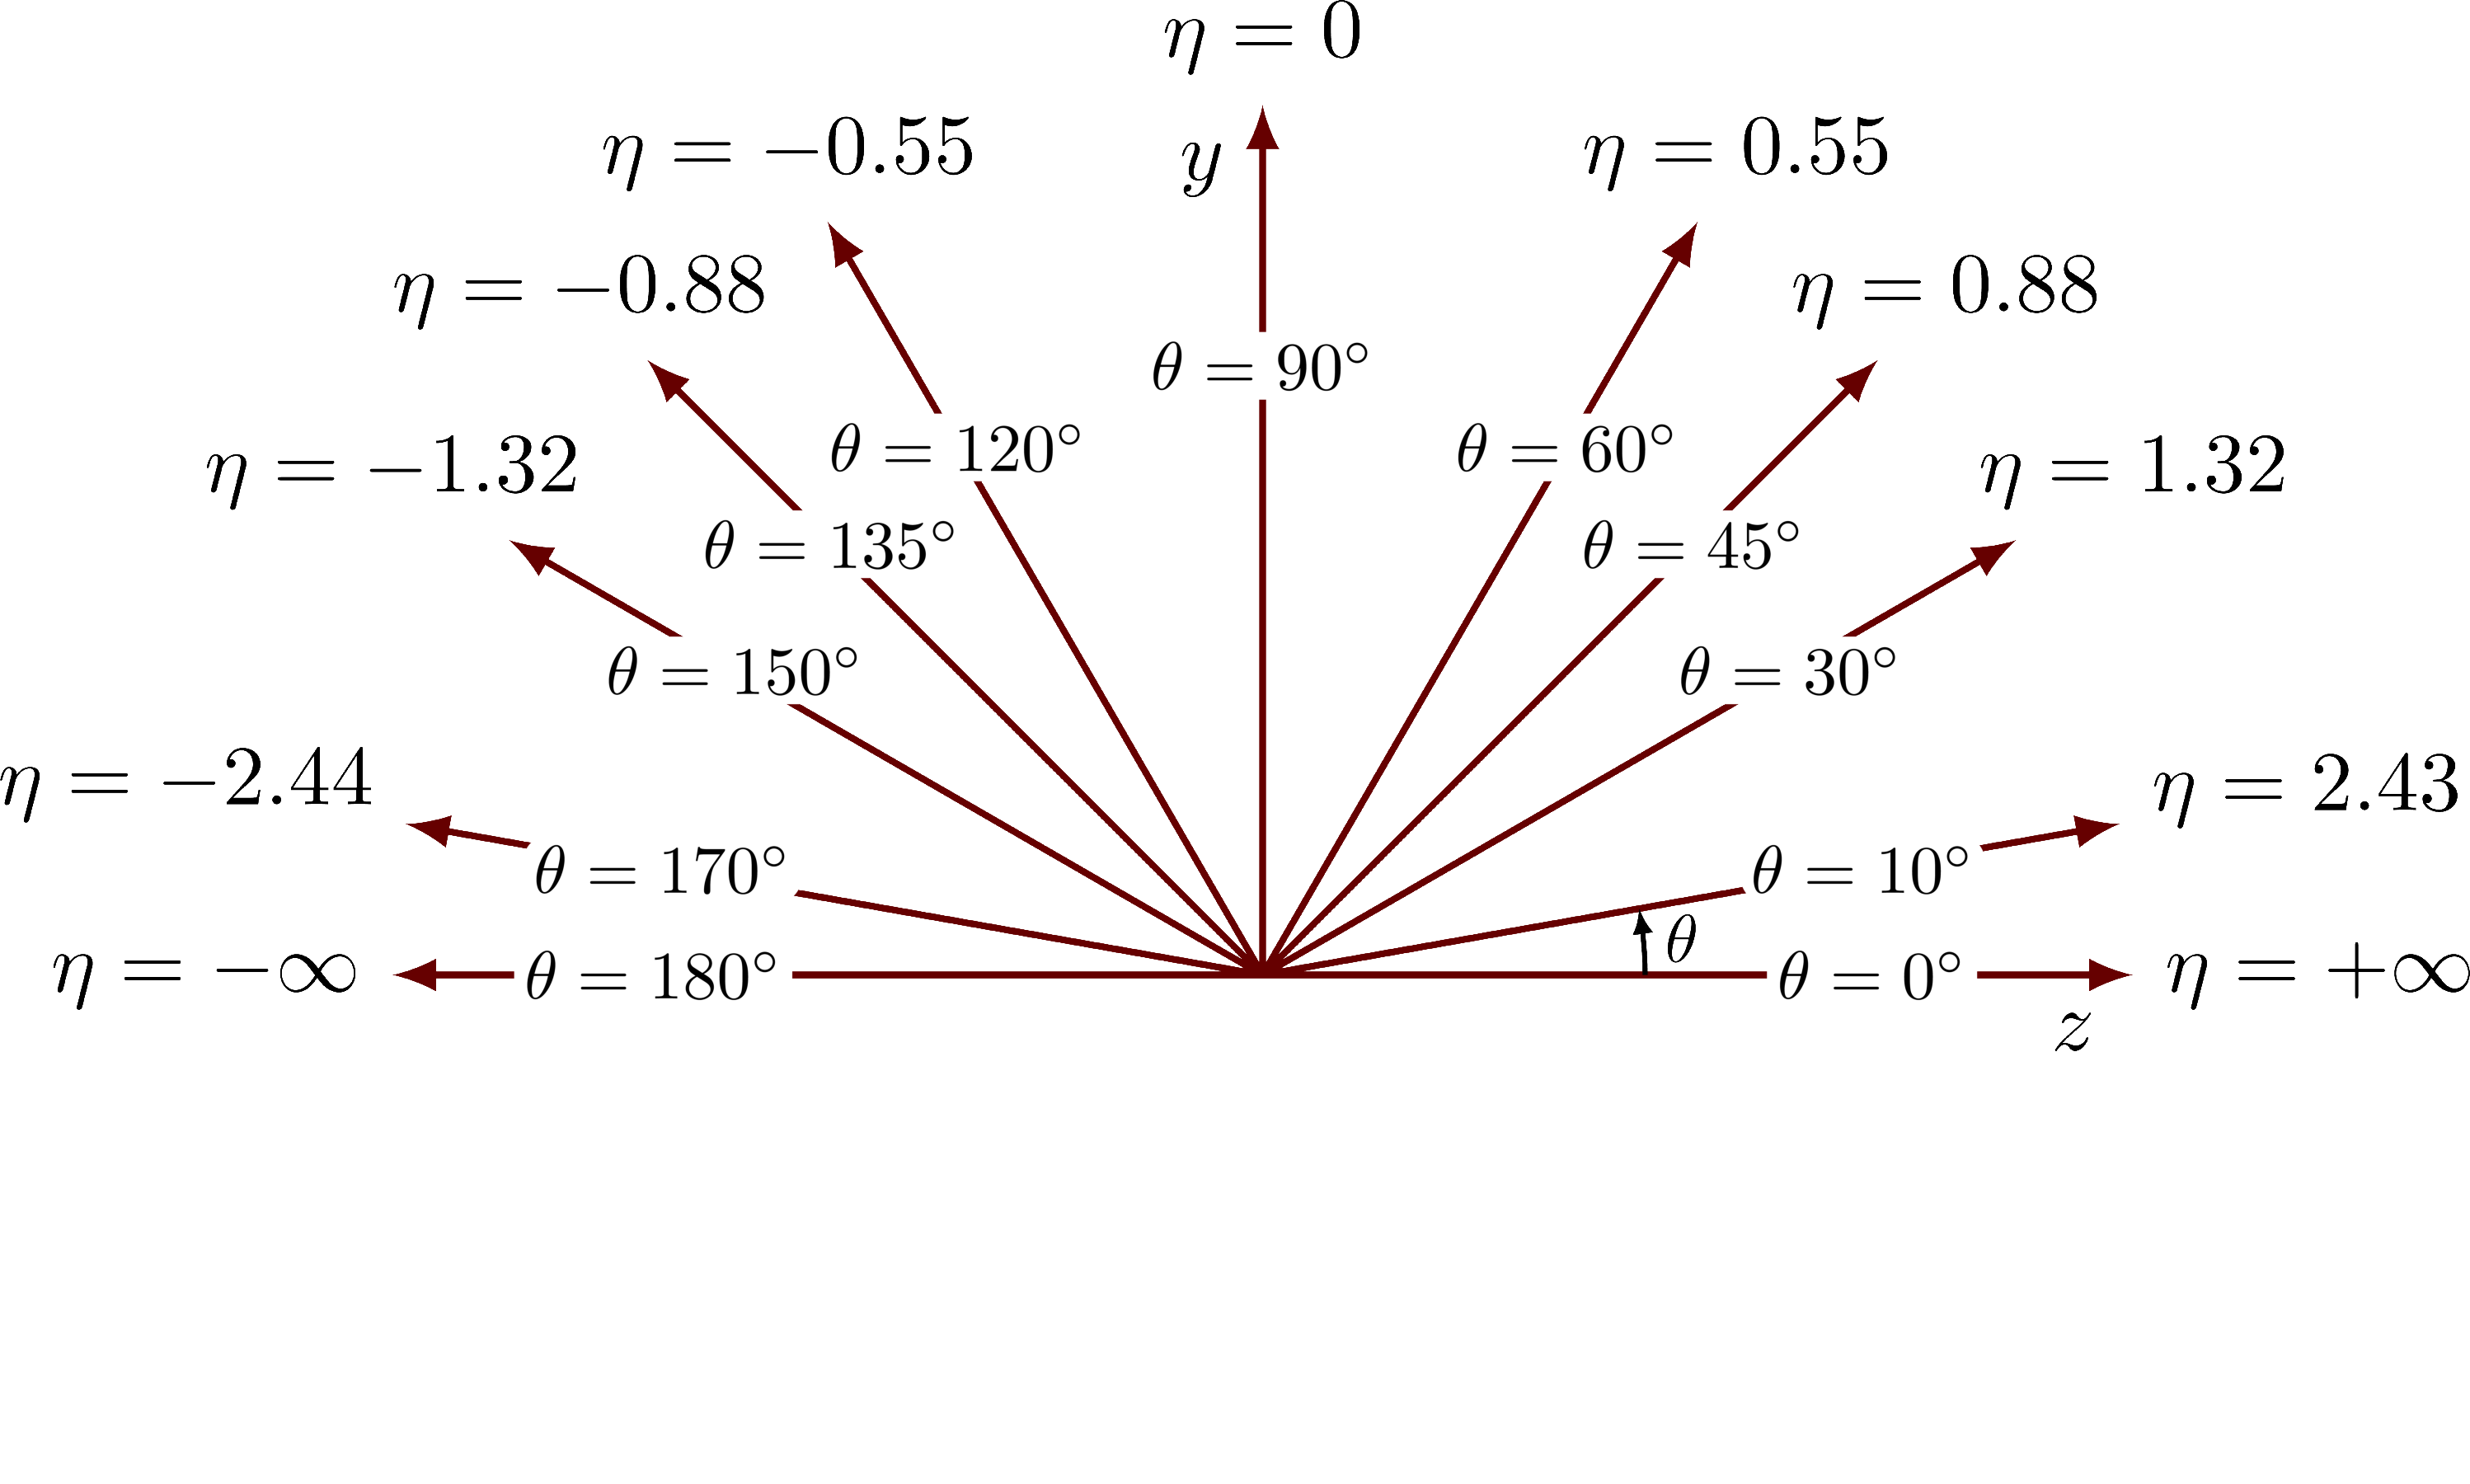
\includegraphics[width=0.8\textwidth]{figures/Part2/CMS/axis2D_pseudorapidity-003}
 \end{tabular}
 \caption{Examples of the conversion between the polar angle $\theta$ and the pseudorapidity $\eta$, adapted from~\cite{tikz:2D}.}
 \label{fig:axis2D}
 \end{center}
\end{figure}

\section{The Tracking system}
\label{sec:TK}

The tracking system~\cite{CMS:1997tlf} is the innermost subsystem of the \ac{CMS} detector where the density of particles from the collisions is the highest. The full Tracking system is based on silicon technology to cope with the high radiation condition and provide excellent spatial resolutions while maintaining a light material budget. The alterations of charged particle trajectories caused by detector materials is expected to be minimal. Hits from charged particles, such as electrons and muons, are measured by silicon sensors and used reconstruct particle trajectories, known as ``tracks''.  The curvature of tracks can be then used to determine the momentum of these final state particles. Tracks can also be used to reconstruct the \ac{PV}, which corresponds to inelastic scatterings in collision events, and the \ac{SV}, which corresponds to the decay of heavy particles, such as tau leptons. 

The Tracking system gives a coverage of up to $|\eta|~<$ 2.5, and is comprised of a pixel detector and a strip detector, which are also collectively known as the tracker detector. When charged particles go through tracker layers, they knocked out electrons in detector materials. These electrons create electric pulses when they travel in electric fields, which are then amplified and detected in the readout electronics. The tracker aims to A sketch of the \ac{CMS} tracker created shortly before Run-1 of the \ac{LHC} is shown in Figure~\ref{fig:Tracker}.

\begin{figure}[tbh!]
 \begin{center}
 \begin{tabular}{c}
 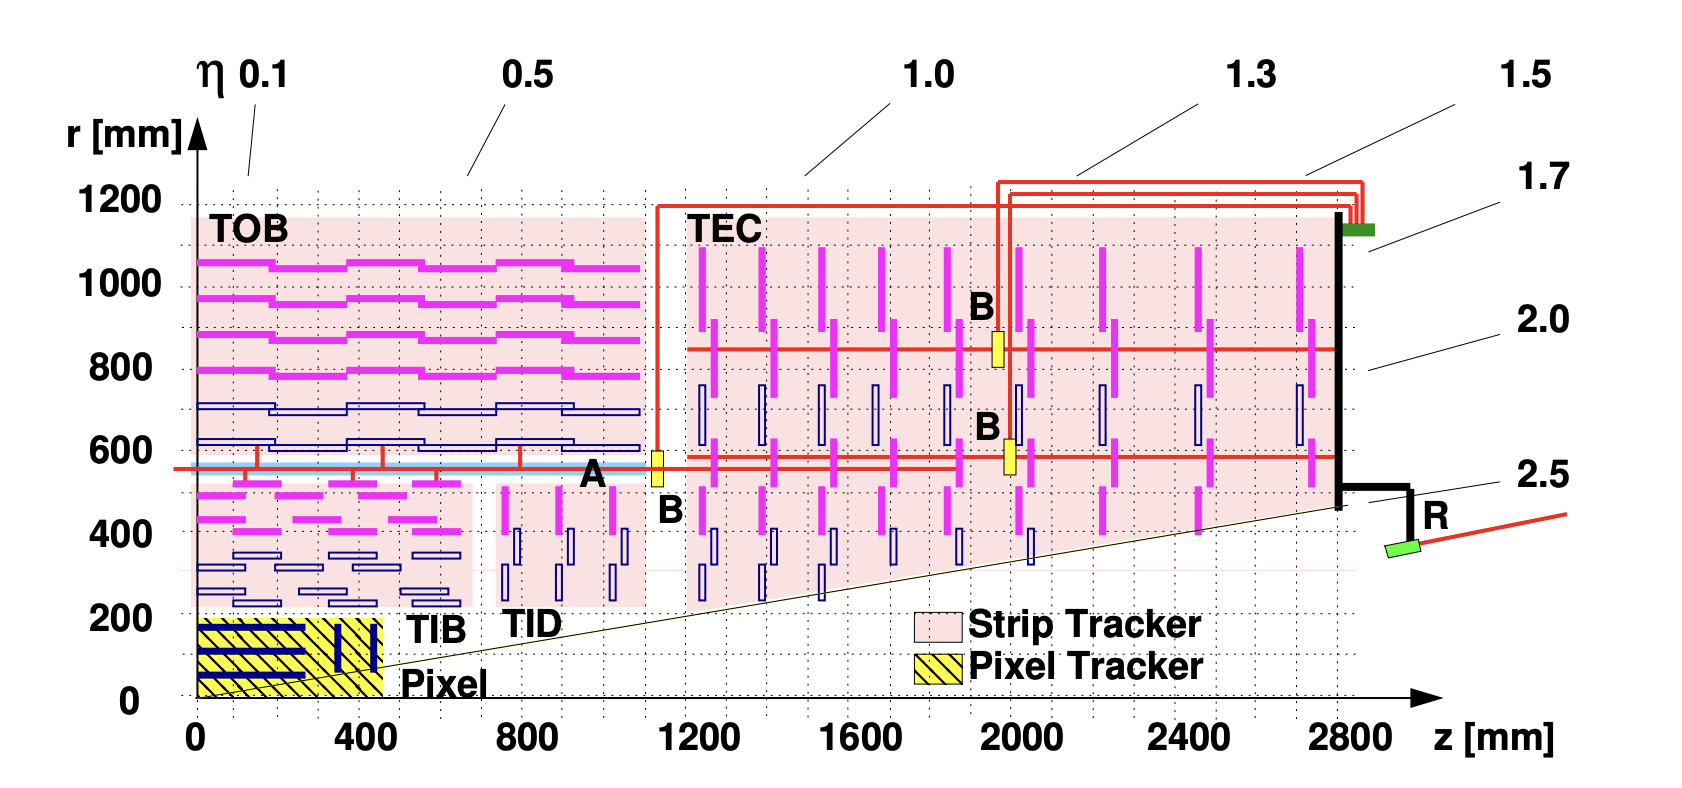
\includegraphics[width=0.8\textwidth]{figures/Part2/CMS/Tracker}
 \end{tabular}
 \caption{Layout of one quadrant of the \ac{CMS} tracker in the $r-z$ plane, adapted from~\cite{CMS:2009dvy}. The strip tracker is shown in pink color while the original pixel detector with three barrel layers is shown in black color.}
 \label{fig:Tracker}
 \end{center}
\end{figure}

The pixel tracker is comprised of roughly 66 million silicon sensors~\cite{CMS:2014pgm}, and is divided into two subsystems: the Barrel Pixel (BPIX) and  Forward Pixel (FPIX). The BPIX is composed of three cylindrical layers with radii ranging from 44 mm to 102 mm. The FPIX is composed of two disks on each side of the forward region. To cope with the intensified \ac{LHC} conditions in Run-2 and improve the overall tracking performance, an upgraded version of the pixel detector, referred to as the Phase-1 pixel detector, was installed during the year-end technical stop between 2016 and 2017~\cite{CMSTrackerGroup:2020edz}. The Phase-1 pixel detector is comprised of roughly 124 million silicon sensors distributed over four BPIX layers and three FPIX disks on each side. Differences between the two pixel detectors are shown in Figure~\ref{fig:Pixel}.

\begin{figure}[tbh!]
 \begin{center}
 \begin{tabular}{c}
 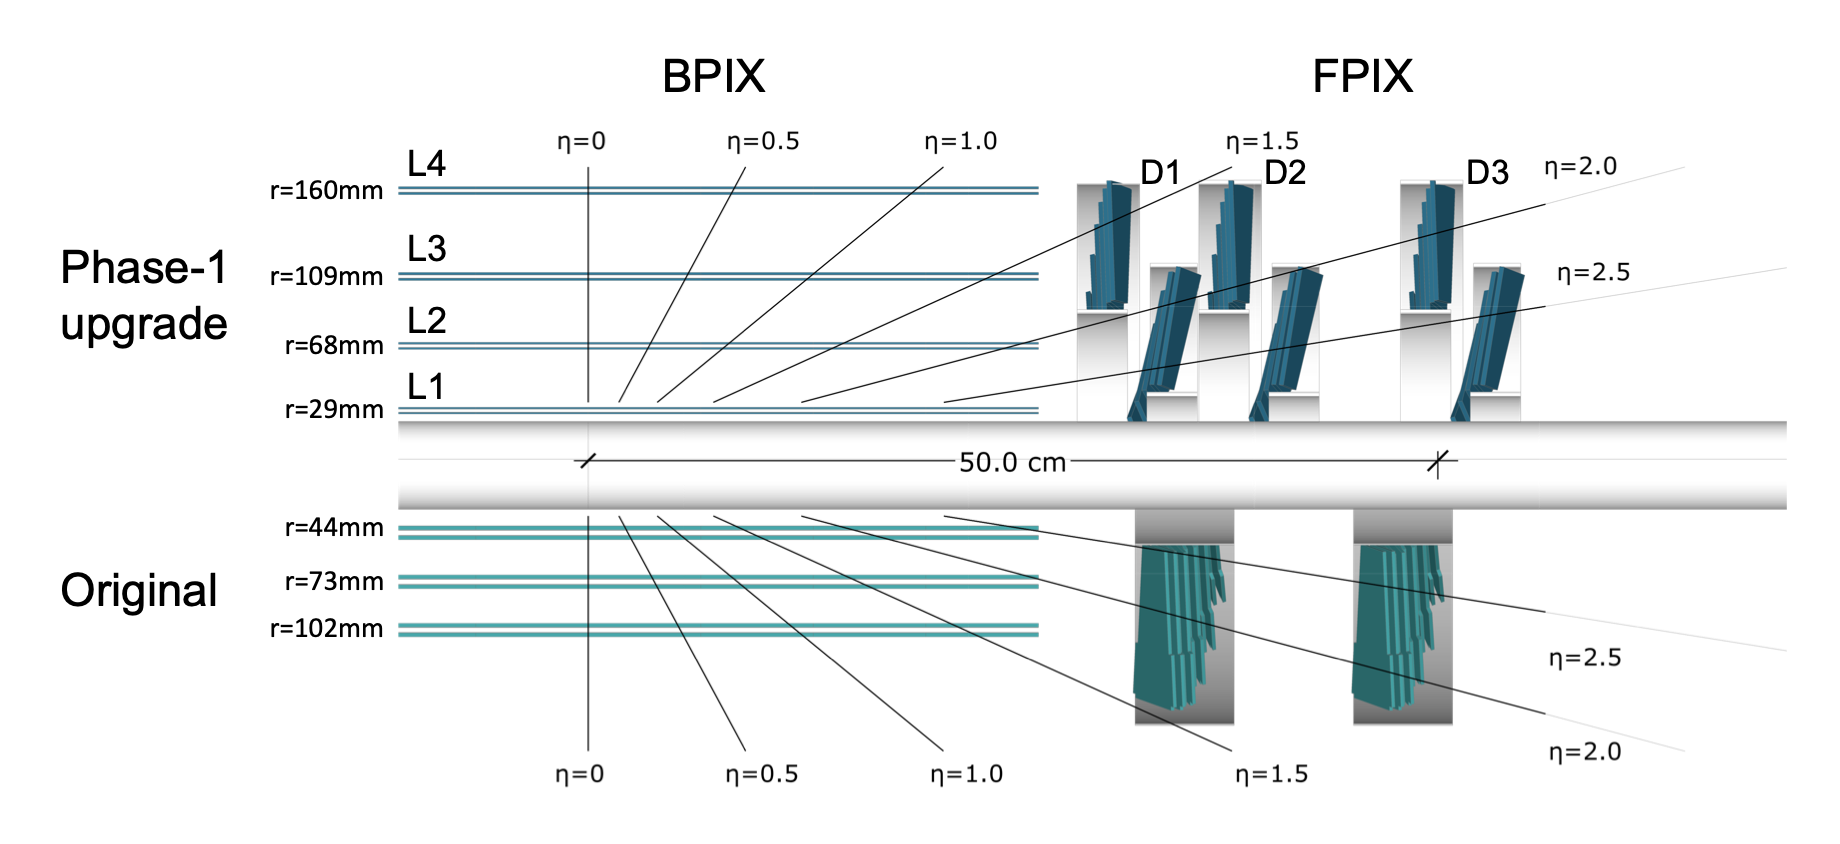
\includegraphics[width=0.85\textwidth]{figures/Part2/CMS/Pixel}
 \end{tabular}
 \caption{A comparison between the original pixel detector and the upgraded pixel detector in the $r-z$ plane, adapted from~\cite{CMSTrackerGroup:2020edz}.}
 \label{fig:Pixel}
 \end{center}
\end{figure}

The strip tracker is much larger in size and is built around the pixel tracker. It is comprised of roughly 10 million silicon sensors and is divided into several subsystems: the tracker inner barrel (TIB), outer barrel (TOB), inner disks (TID), and endcaps (TEC). The TIB and TOB consist of four and six layers, respectively. The TID and TEC consist of three and nine disks, respectively.

\section{The Electromagnetic Calorimeter}
\label{sec:ECAL}

The \ac{ECAL}~\cite{CMS:1997ysd} is homogeneous calorimeter that encloses the tracker detector, and thus it is the second innermost subsystem of the \ac{CMS} detector. It helps determine the energy and position of electrons and photons through their electromagnetic interactions with detector materials. The \ac{ECAL} gives a coverage of up to $|\eta|~<$ 3.0, and is divided into three subsystems: the \ac{ECAL} barrel calorimeter (EB), preshower calorimeter (ES), and endcap calorimeter (EE). A sketch of the \ac{ECAL} layout is shown in Figure~\ref{fig:ECAL}.

\begin{figure}[tbh!]
 \begin{center}
 \begin{tabular}{c}
 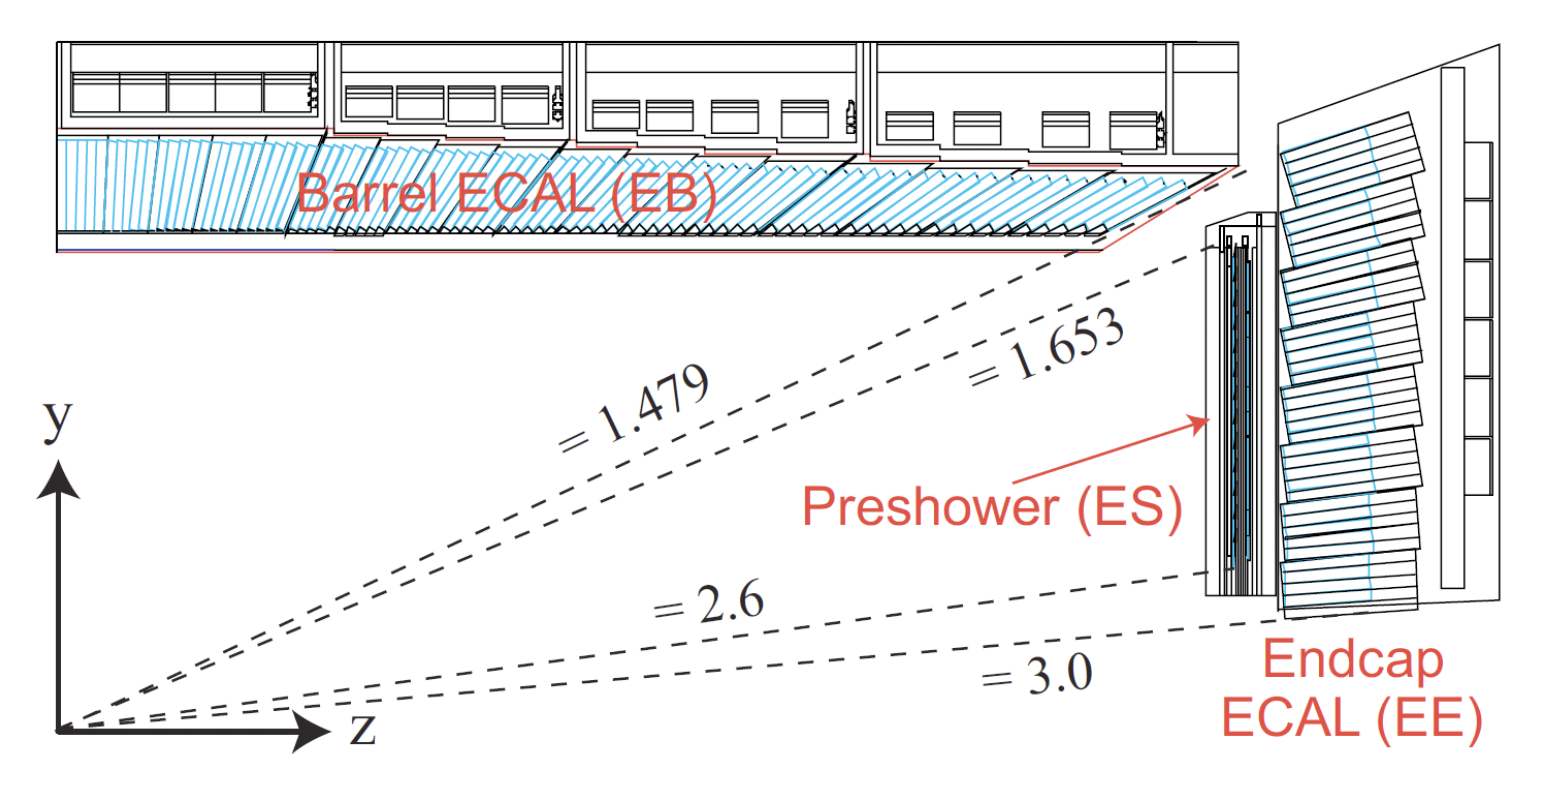
\includegraphics[width=0.8\textwidth]{figures/Part2/CMS/ECAL}
 \end{tabular}
 \caption{Layout of one quadrant of the \ac{ECAL} in the $r-z$ plane, adapted from~\cite{Benaglia:2014aqa}.}
 \label{fig:ECAL}
 \end{center}
\end{figure}

Unlike the tracker, the \ac{ECAL} aims to stop electrons and photons entirely. It is composed of over 76 thousand lead tungstate (PbWO$_{4}$) crystals, which act as absorber and scintillator simultaneously. When high-energy electrons and photons travel through these crystals, they create electromagnetic showers of low-energy electrons and photons. Over 98 \% of the shower energy can be absorbed and converted to light through the scintillation process. The scintillation light is then amplified and detected by photodiodes. The energy of particles can be measured from the intensity of the scintillation light.

\section{The Hadronic Calorimeter}
\label{sec:HCAL}

The \ac{HCAL}~\cite{CMS:1997xji} is a sampling calorimeter placed outside of the \ac{ECAL}. It measures the energy of hadrons through their strong interactions with detector materials. It also plays a crucial role in the measurement of the total energy in collision events, which allows for the determination of the \ac{MET}. The \ac{HCAL} gives a coverage of up to $|\eta|~<$ 5.2, and is divided into four subsystems: the \ac{HCAL} barrel calorimeter (HB), endcap calorimeter (HE), outer barrel calorimeter (HO), and forward calorimeter (HF). A sketch of the \ac{HCAL} layout is shown in Figure~\ref{fig:HCAL}.

\begin{figure}[tbh!]
 \begin{center}
 \begin{tabular}{c}
 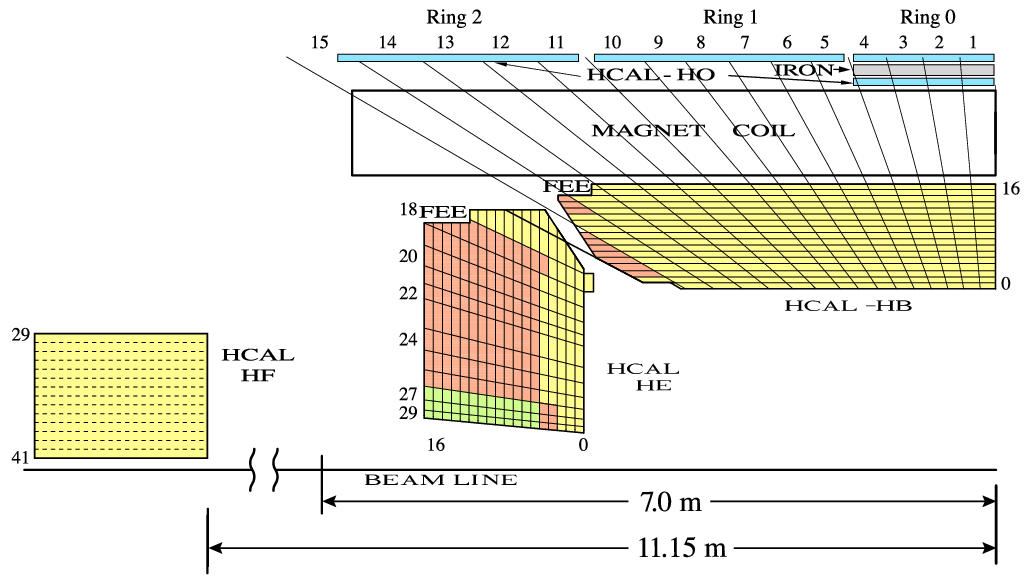
\includegraphics[width=0.9\textwidth]{figures/Part2/CMS/HCAL}
 \end{tabular}
 \caption{Layout of one quadrant of the \ac{HCAL} in the $r-z$ plane, adapted from~\cite{CMS:2009nwd}.}
 \label{fig:HCAL}
 \end{center}
\end{figure}

Similar to the \ac{ECAL}, the \ac{HCAL} aims to stop hadrons entirely as their momenta are only minimally affected by the tracker and \ac{ECAL}. Unlike the \ac{ECAL}, which is homogeneous in its detector materials, the \ac{HCAL} uses alternating layers of absorbers and scintillators made of different materials and hence it is classified as a sampling calorimeter. Brass absorber plates are placed between plastic scintillators plates in the HB and HE, which provides coverages of $|\eta|~<$ 1.3 and 1.3 $<~|\eta|~<$ 3.0, respectively. The HO is placed outside of the magnetic coil to provide additional materials in barrel. It uses materials from the \ac{CMS} magnet as absorbers. The HF is placed outside of the detector around the beam line. It provides coverage of forward jets and uses steel as absorbing materials. 

\section{The Superconducting Magnet}
\label{sec:Magnet}

The superconducting magnet~\cite{CMS:1997moj} is the central feature of the \ac{CMS} detector. It has a diameter of roughly 6 meters and full encloses the tracker, \ac{ECAL} and the \ac{HCAL} HB and HE. The magnet consists of two main parts: the steel return yoke and the superconducting solenoid. The yoke weights more than 10 thousand tons and its main role is to improve the homogeneity of the magnetic filed inside the tracker and return the magnetic flux to the solenoid. The superconducting solenoid is enclosed in the yoke and it produces a uniform magnetic field of $B~=~3.8$ T inside the tracker volume. The paths of charged particles are curved by this magnetic field so that their momenta can be inferred from the curvatures of the trajectories according to the equation

\begin{equation}
\pt = |q|B\rho,
\end{equation}

where $q$ is the charge of the particle, $B$ is the magnetic field in the z direction, and $\rho$ is the radius of the curvature. A map of  the magnetic field generated by the solenoid is shown in Figure~\ref{fig:Magnet}. The solenoid operates at a current of over 18 thousand A and a temperature of 4.2 K (-268.95 $^\circ$C). It is cooled by the liquid helium.

\begin{figure}[tbh!]
 \begin{center}
 \begin{tabular}{c}
 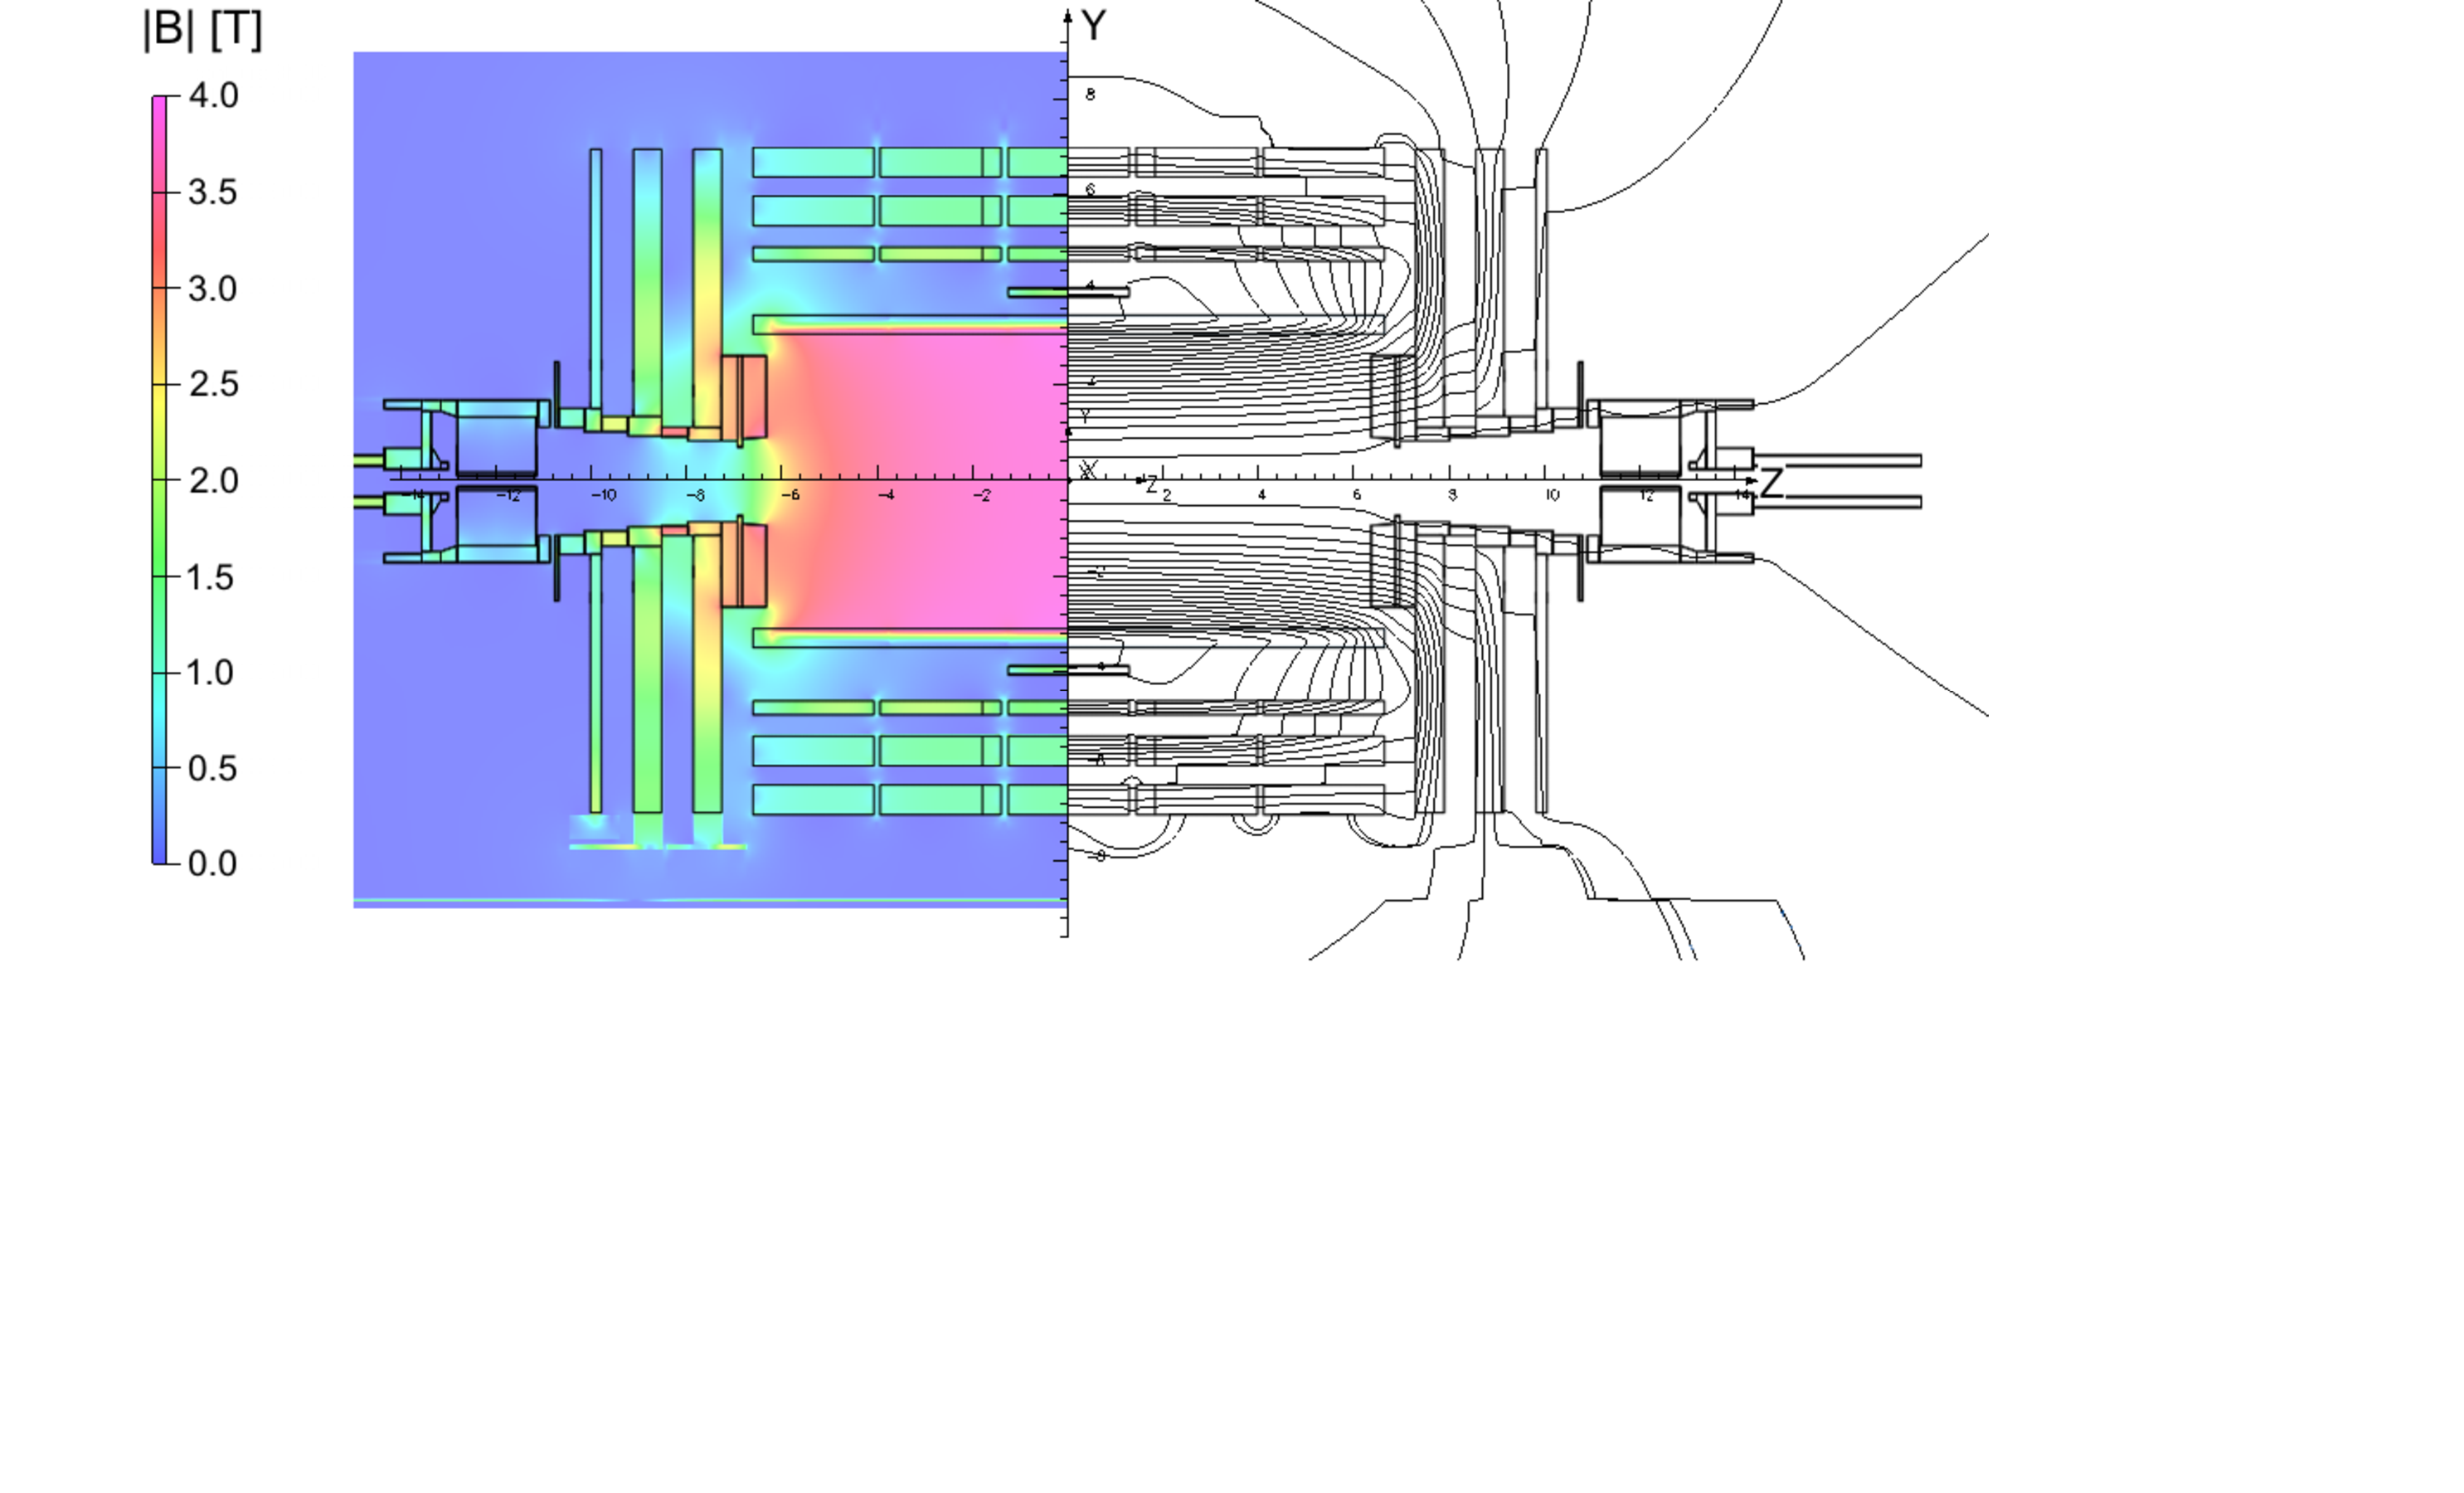
\includegraphics[width=0.8\textwidth]{figures/Part2/CMS/Magnet}
 \end{tabular}
 \caption{Predicted values of $|B|$ (left) and field lines (right) on a longitudinal section of the \ac{CMS} detector, adapted from~\cite{CMS:2009moq}.}
 \label{fig:Magnet}
 \end{center}
\end{figure}

\section{The Muon System}
\label{sec:MuonSys}

The Muon system~\cite{CMS:1997iti} is located outside of the solenoid and embedded into the return yoke. It is the outermost and largest subsystem of the \ac{CMS} detector, consisting of several subsystems that give an overall coverage of up to $|\eta|~<$ 2.4. All these subsystems all based on gas-ionization technology: the \ac{DT} and \ac{RPC} together make up the barrel region of the Muon system, and the endcap Muon system consists of \ac{RPC} and  \ac{CSC}. The \ac{GEM}~\cite{Colaleo:2015vsq} is the latest addition to the Muon system. It complements \ac{CSC} in the forward region. A sketch of the Muon system layout is shown in Figure~\ref{fig:Muon}.

\begin{figure}[tbh!]
 \begin{center}
 \begin{tabular}{c}
 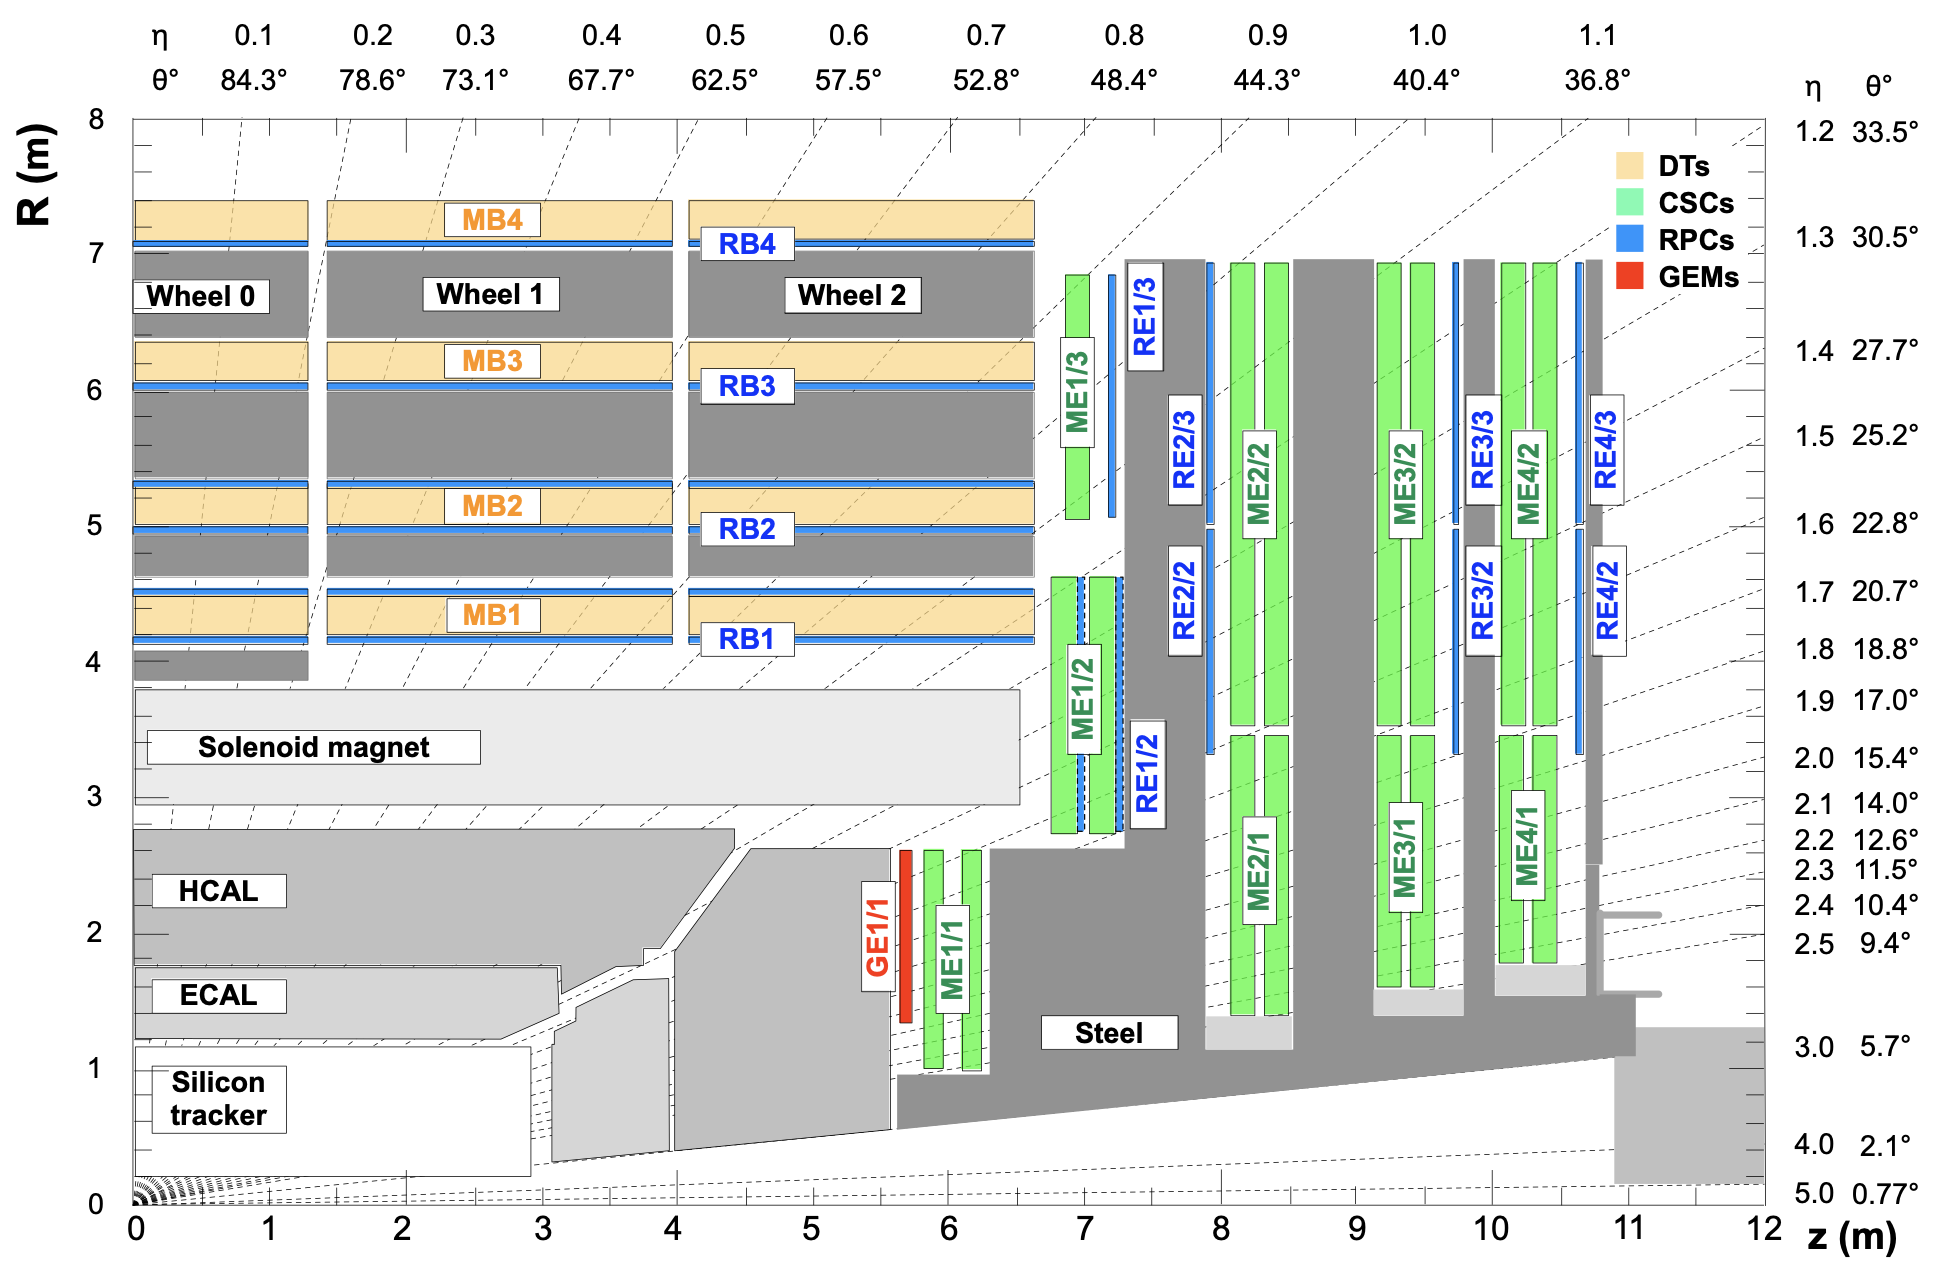
\includegraphics[width=1\textwidth]{figures/Part2/CMS/Muon}
 \end{tabular}
 \caption{Layout of one quadrant of the Muon system in the $r-z$ plane, adapted from~\cite{Colaleo:2015vsq}.}
 \label{fig:Muon}
 \end{center}
\end{figure}

Muons produced in collision events retain most of their momenta when they penetrate the tracker and calorimeters, which allows for the precise determination of their trajectories by the Muon system. The barrel region ($|\eta|~<$ 1.2) is occupied by four stations of \acp{DT}, which consists of charged wires and is filled with gas. The \ac{DT} is chosen for this region because the event rate is lower in this region and magnetic field is weaker but more uniform relative to the forward region. When muons pass through the \ac{DT} chambers, they knock out electrons from the gas atoms, which then move towards the positively charged wires due to its electric field. The charged wires are placed perpendicular to each other so that the $x$ and $y$ coordinates of the muon positions can be determined. 

In region (0.9 $<~|\eta|~<$ 2.4) where event rate is higher, four stations of the \ac{CSC} chambers are positioned on each side. Similar to the detection mechanism in the \ac{DT}, muons knock out electrons from gas atoms when they pass through the \ac{CSC} chambers. Unlike the \ac{DT}, which solely relies on positively charged wires, the \ac{CSC} uses positively charged wires and negatively charged strips positioned perpendicular to each other. When electrons move to the wires, they create an avalanche of electrons. At the same time, a signal in the strips will be created by the ionized gas atoms. These two signals together allows for the determination of the $x$ and $y$ coordinates of the muon positions. 

Complementary to the \ac{DT} and \ac{CSC}, the \ac{RPC} chambers are positioned in both barrel and endcap region ($|\eta|~<$ 1.9). They provide coarser position resolution but fast response and good time resolution, which is useful in the muon trigger. The \ac{GEM} will extend the coverage of the Muon system to $|\eta|~<$ 2.8 and is expected to be fully operational before the start of the Run-4. 

\section{The Trigger System}
\label{sec:TrigSys}
 
The \ac{LHC} collides proton bunches every 25 ns, which corresponds to an event rate of 40 MHz. The size of the data generated at this collision rate is too large and it is beyond the hardware limit to record every event offline. Moreover, vast majority of the events involve only soft \ac{QCD} processes that is of little interests to particle physicists. The \ac{CMS} trigger system~\cite{CMS:2016ngn} is designed to reduce the data volume to a feasible level and select events that are interesting to the physics programs at the \ac{CMS}. It consists of two layers: the \ac{L1} trigger and \ac{HLT}.

The \ac{L1} trigger is the first layer of the trigger system and is based on custom-designed hardware. Before high resolution collision events are recorded permanently, they are held in memory pipelines at the frontend electronics. The \ac{L1} trigger is tasked to analyze every event by only coarsely using the segmented data from the calorimeters and the Muon Systems, as illustrated in Figure~\ref{fig:L1T}. It makes an irreversible decision on which events to keep and which events to discard in less than 4 $\mu$s and reduces the event rate to about 100 kHz.

\begin{figure}[tbh!]
 \begin{center}
 \begin{tabular}{c}
 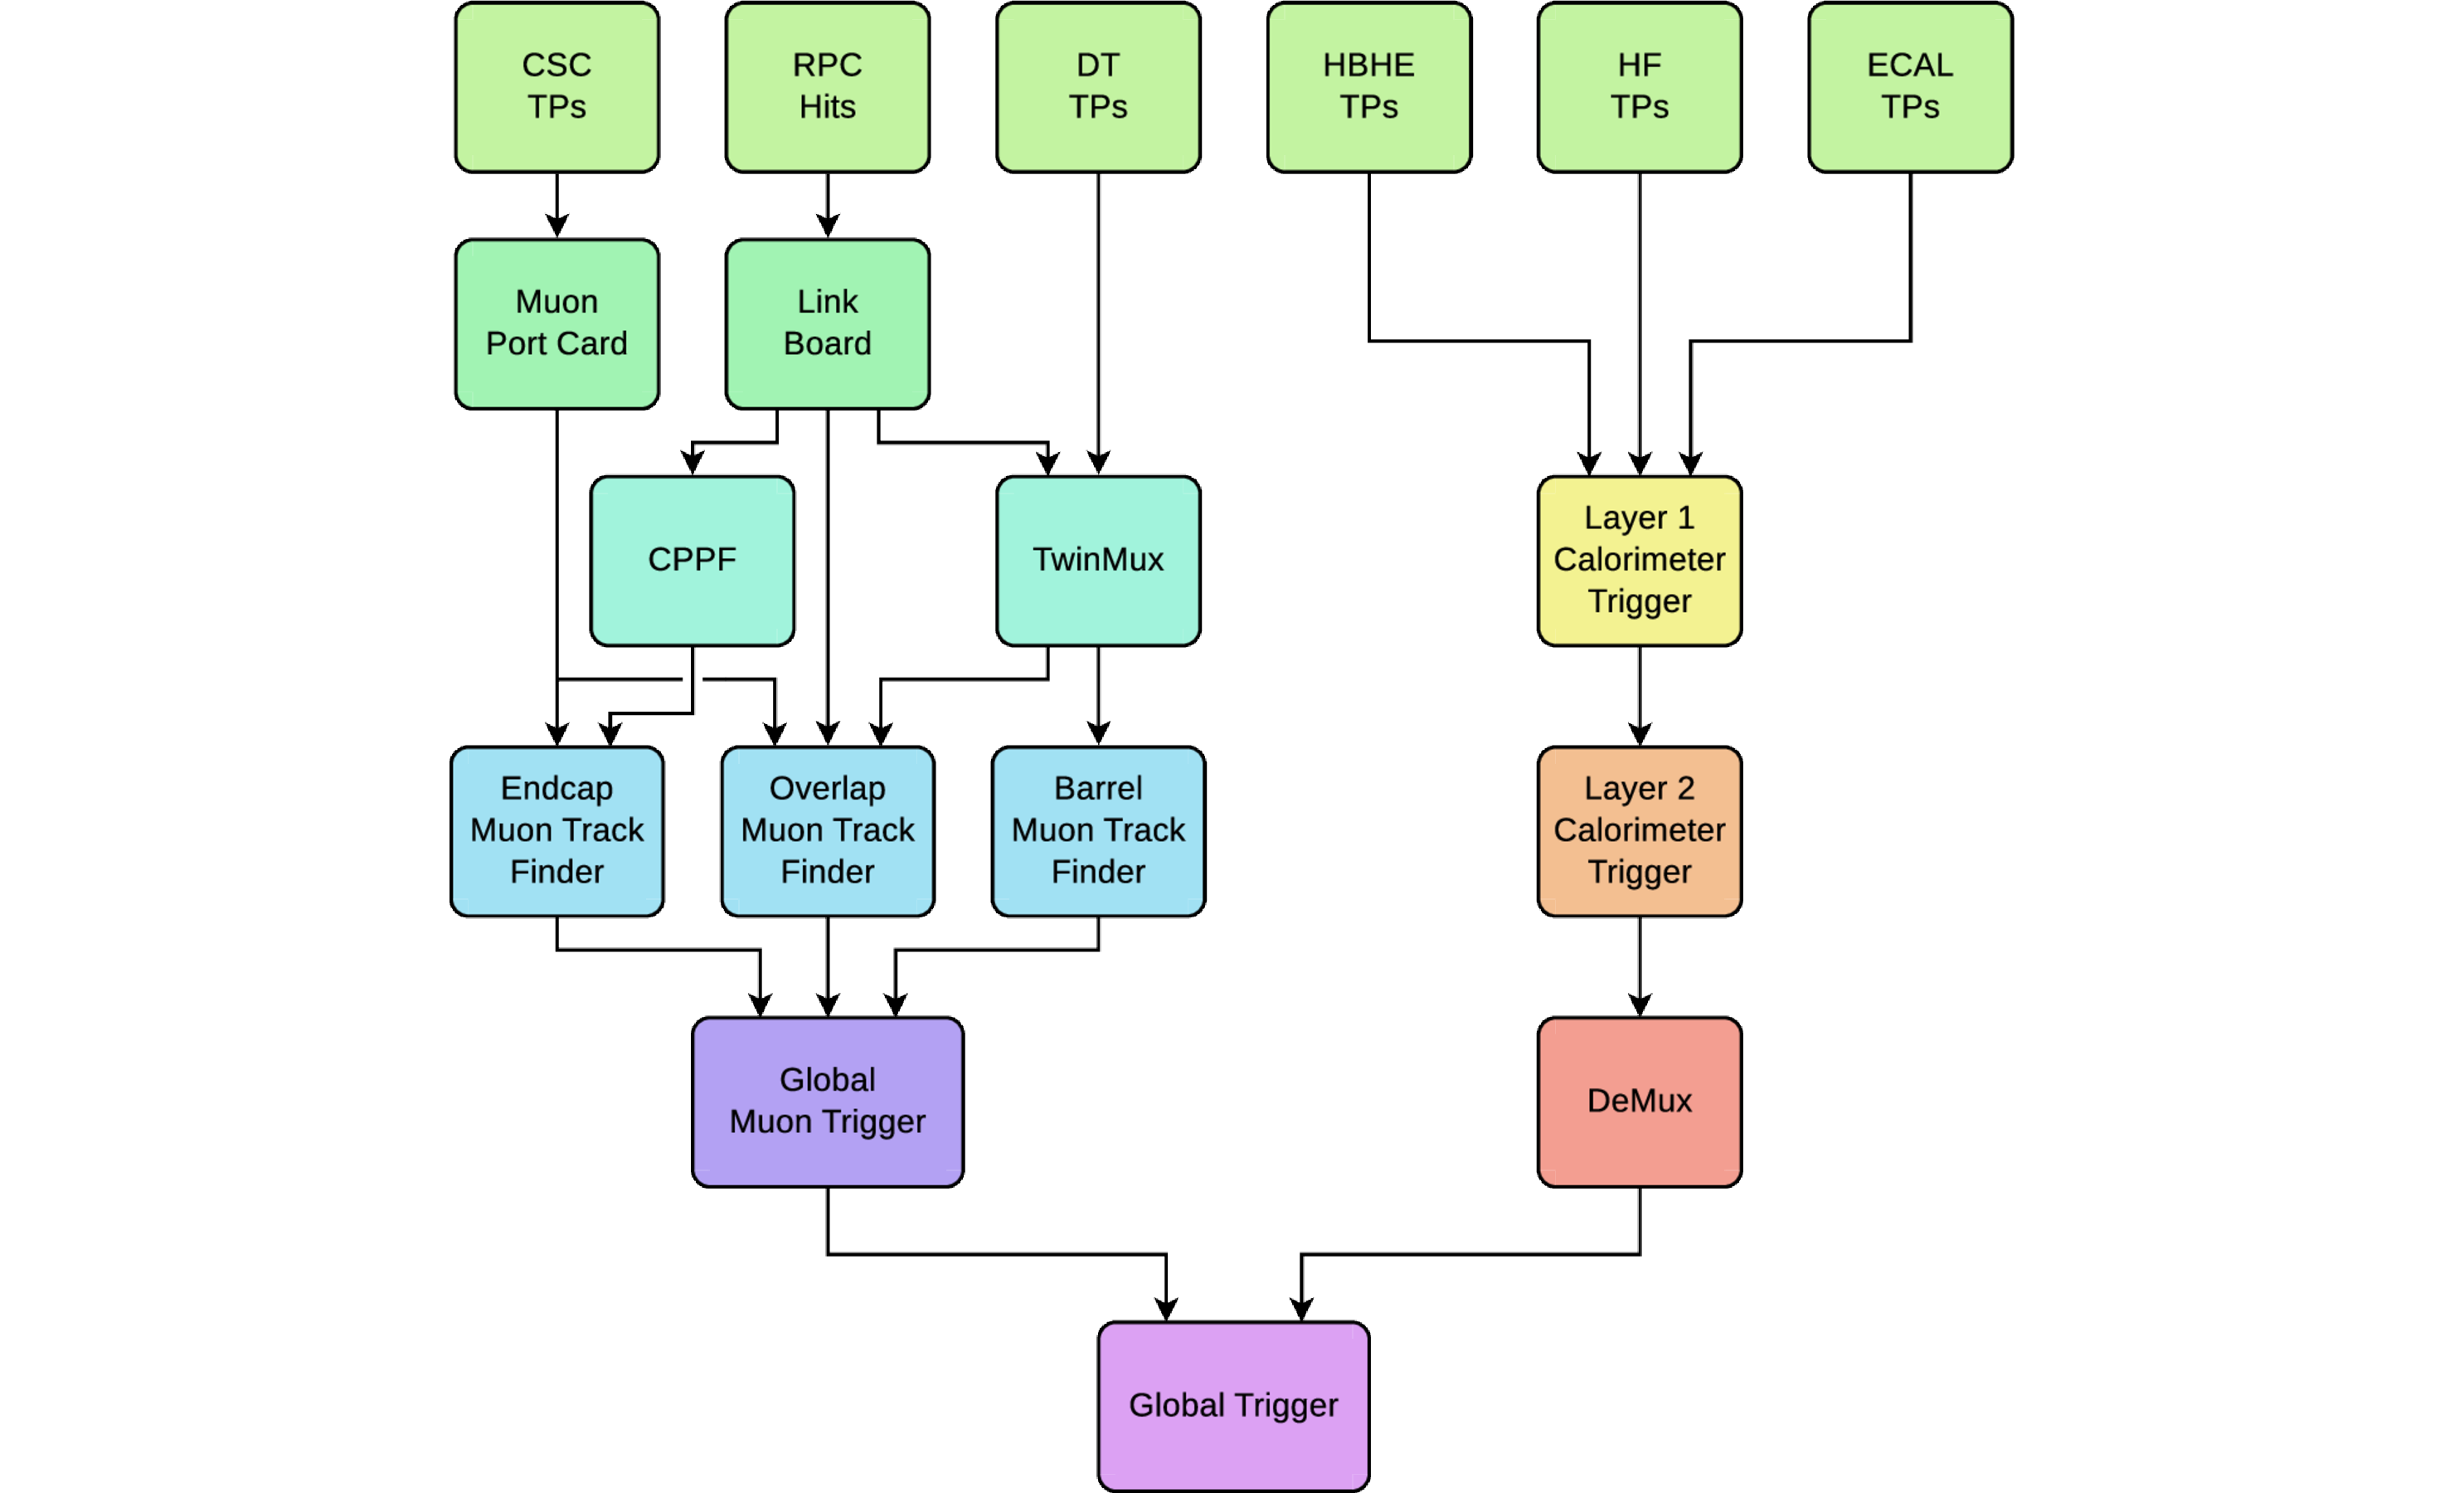
\includegraphics[width=1\textwidth]{figures/Part2/CMS/L1T}
 \end{tabular}
 \caption{Diagram of the \ac{L1} trigger system during Run-2 of the \ac{LHC}, adapted from~\cite{CMS:2020cmk}.}
 \label{fig:L1T}
 \end{center}
\end{figure}

Before the start of the Run-2, an upgraded version of the \ac{L1} trigger~\cite{Tapper:2013yva} was installed. This upgraded \ac{L1} trigger adds additional layers of correlators between the muon trigger and calorimeter trigger, which allows for more advanced computations such as the muon isolation. 

The \ac{HLT} is the second layer of the trigger system and is based on a software-based algorithms that run on computer farms. Unlike the \ac{L1} trigger, the \ac{HLT} has access to the full readout data, which allows for the deployment of more sophisticated algorithms to select events targeted by different physics groups. The event rate is further reduced by the \ac{HLT} selection to about 400 Hz.